\documentclass{nime-alternate} % Uncomment when publishing final version

% Uncomment only one of the ones below
% \usepackage{anonymize} 		   %Uncomment this line to publish
\usepackage[blind]{anonymize}%Uncomment this line for blind review

% Package that enables the use of accents and non 
% standard characters
\usepackage[utf8]{inputenc}

\begin{document}

\conferenceinfo{NIME'24,}{4--6 September, Utrecht, The Netherlands.}
\title{Step-by-Step: Training IMU-based Gestures with Live Feedback}


\label{key}

\numberofauthors{1} 

\author{
% 1st. author
\alignauthor
\anonymize{Michael Schnebly}\\
       \affaddr{\anonymize{School of Engineering and Applied Sciences}}\\
       \affaddr{\anonymize{Harvard University}}\\
       \affaddr{\anonymize{Cambridge, MA, USA}}\\
       \email{\anonymize{michael\_schnebly@g.harvard.edu}}
}
% For your initial submission you MUST ANONYMIZE the authors.

\maketitle
\begin{abstract}
This document serves as an application to NIME's 2024 Student Consortium. Within it, I present my interest in joining the NIME research community, as well as my preliminary results for \textit{Step-by-Step}, a software tool that allows users to train gesture recognition models with live audiovisual feedback. \textit{Step-by-Step} uses a simple neural network to learn to recognize and distinguish multiple gestures in inertial measurement unit (IMU) timeseries data. Users train the model by repeatedly performing a target gesture while receiving live feedback on the model’s ability to recognize that gesture. Once satisfactory results are achieved, the user can save the model and deploy it for realtime musical applications, as demonstrated in supplementary live performance videos. An anonymized code repository is available at \url{https://anonymous.4open.science/r/step-by-step-7506/}
\end{abstract} 
\keywords{Gesture Recognition, IMU, Real-time, Neural Network, Training, Inference, Live Feedback}
\ccsdesc[300]{Applied computing~Sound and music computing}
\ccsdesc[300]{Human-centered computing~Gestural input}
\ccsdesc[300]{Machine learning~Neural networks}

% this line creates the CCS Concepts section.
\printccsdesc

\section{Expected Outcomes}

\section{Introduction}
The broad range of possible mappings between body movement and sound afforded by gesture-based digital musical instruments presents the musician with a creative challenge: Which body movements? Which sounds? And, what is the mapping between them \cite{mitchell:mapping}?

A common approach to this challenge are \textit{learned} mappings, for which the musician records themselves demonstrating a gesture, then trains a machine learning model to recognize and distinguish the target gesture from other body movements. Indeed, the NIME community has produced several software tools that facilitate this process \cite{bullock:mllib,fiebrink:wekinator, gillian:toolkit, caramiaux:nimeml, mcpherson:pipeline}.

These interactive machine learning tools are typically designed for offline training, wherein the musician records training data, trains the model, then tests it. With no knowledge of how the model will perform until after training, the musician must iterate, repeatedly recording, training, and testing until a satisfactory result is achieved. This opaque, iterative process can be a hindrance to creative flow, especially in live performance settings where improvising novel gesture-sound mappings might be desirable.

Ideally, one would be able to train a model in realtime, receiving live feedback on the model's performance as it learns each time a gesture is performed. Receving model performance reports on a per-gesture basis, the musician can build intuition for what the model has learned (e.g. which variations on the gesture are recognized and whicvh are not), adjust their gesture demonstrations accordingly, and arrive at a satisfactory result more efficiently.

This is the motivation behind \textit{Step-by-Step}, a software tool that allows users to train gesture recognition models with live audiovisual feedback. Here we present the system's hardware and software components, the method by which they are integrated, and preliminary results demonstrating the system's ability to learn to recognize and distinguish gestures in realtime.

\section{Background}
\subsection{Gesture Recognition}
Gesture recognition is the process of recognizing and distinguishing gestures in data. Gestures are body movement patterns that convey information. In the context of digital musical instruments, gestures are often used to control sound. For example, a musician might use a gesture to control the pitch of a note, the volume of a sound, or the timbre of an instrument.

\subsection{Inertial Measurement Units}
Inertial measurement units (IMUs) are one of many types types of sensors that can be used to measure body movement. IMUs typically include an accelerometer, gyroscope, and magnetometer, each of which measures in three axes: x, y, and z. IMUs are commonly used in wearable devices to track body movements over time. In this work, we use IMUs to measure body movement and recognize gestures.

\subsection{Neural Networks}
Neural networks are one of many classes of machine learning models that can be used to analyze IMU timeseries and identify patterns such as gestures. In \textit{supervised learning}, neural networks are trained by providing them with examples of inputs and corresponding correct output labels. During training, the model adjusts its parameters to minimize the difference between its predictions and the groundtruth outputs. This process is called gradient descent and is performed iteratively until the model converges on a solution. Once trained, the model can be used to make predictions on novel inputs. Here, we perform gradient descent in parallel to the recording and automated labelling of training data, allowing the model to learn in real-time as new examples are provided.

\section{Method}
The system consists of hardware and software components. The hardware measures body movement and streams the data to a computer. The software processes the data, trains a neural network, and provides live feedback to the user. The system is designed to be accessible to users with no machine learning experience while providing a powerful codebase for advanced users.

\subsection{Hardware}
For measuring body movement, we used the Bosch BNO-055, a 9-axis IMU that includes an accelerometer, gyroscope, and magnetometer. The IMU uses I2C communication protocol to stream data to a microcontroller (Espressif ESP8266) which passes that data on to a laptop  (Macbook Pro 2017) via USB for further processing.

Note that the particular hardware components used in this project are not essential to the system. They could be replaced with other options so long as the sensor data contains information necessary to recognize and distinguish the gestures of interest and the computer (or microcontroller if using purely embedded approach) is capable of running the software at a rate matching that of data collection.
% The hardware is shown in Figure \ref{fig:hardware}.

\subsection{Software}
The software is written in Python and structured into three main components: data processing, neural network, and user interface. The data processing component handles data collection, labelling, and storage. The neural network component handles model structure, training, and inference. The user interface component handles user interaction and feedback.

To facilitate realtime training and inference, the software is structured as a pipeline with the following processes running in parallel: data processing, model training, and model inference. Importantly all processes refer to the same global variables, allowing them to share updates to the model and training data in realtime.
% The software architecture is shown in Figure \ref{fig:software_architecture}.


\begin{figure}[h]
    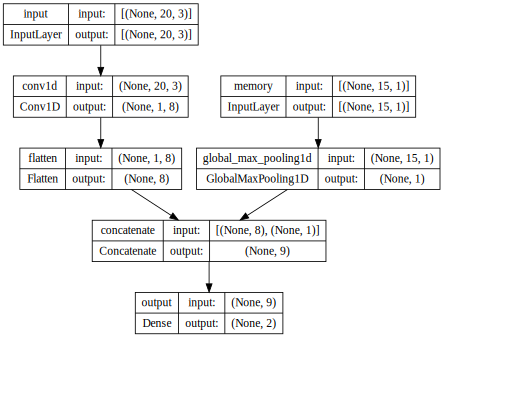
\includegraphics[width=0.5\textwidth]{../figures/model_diagram.jpg}
    \caption{Neural Network Architecture. The sensor branch (left) receives 20 frames (200 ms at 100 Hz) of 3-channel (x, y, z) IMU data. The sensor branch feeds into a 1D-convolutional layer with 8 filters, each also 20 frames in width. The memory branch (right) receives 15 frames of 1-hot encoded prediction data. The two branches are concatenated and fed into a fully connected output layer to predict the currently active gesture.}
    \label{fig:neural_network}
\end{figure}


\subsection{Data Processing}
\subsubsection{Collection}
The IMU data is collected as a timeseries of frames. Each frame is a 3D vector representing linear acceleration in each of the three axes: x, y, and z. The data is collected at a rate of 100 Hz and can be streamed directly from an IMU, recorded to a file, or loaded from a file.

\subsubsection{Labelling}
The data is labelled by associating each frame with a gesture. A gesture is a sequence of frames that represents a single movement of the body. Here, we focus on percussive gestures and assume that a gesture is complete at the local peak in linear acceleration's magnitude. This constraint allow us to achieve realtime, automated labelling of gestures using a simple peak-detection algorithm. When a local peak meet's user-defined criteria (e.g. acceleration is above a certain threshold), the peak frame is labelled as containing a gesture. All other frames are labelled as containing no gesture.


\begin{figure*}[h]
    \centering
    \includegraphics[width=1.0\textwidth]{../figures/realtime_training.jpg}
    \caption{Live Learning Feedback: The user performs a gesture and receives live feedback on the model's performance. Bottom Panel: 10 seconds of training data. Acceleration components (x, y, z) are shown in color; magnitude is shown in grey. Each magnitude peak is marked by a thin vertical line, indicating it has been labelled as a gesture in the training data. Top Panel: 10 seconds of inference data. At t = 0 seconds the neural network is completely untrained. Naive to what is and is not a gesture, it predicts gesture and non-gesture with equal probability (0.5). As the model trains on non-gesture date, it begins to predict non-gesture with higher probability. At t = 5 seconds, the model has converged on a solution that reliably distinguishes non-gesture. At t = 10 seconds, the model has converged on a solution that reliably distinguishes gestures. Given more training data and time to learn, the model's performance would continue to improve with gessture and non-gesture probabilities approaching 1 and 0, respectively. See supplementary video for live demo in the github repo.}
    \label{fig:realtime_training}
\end{figure*}

\subsection{Neural Network}
\subsubsection{Structure}
The neural network is a shallow, two-branched model. One branch represents a recent history of sensor values while the other represents a recent history of model outputs. Combining the information from the these two sources, the model is trained to maximize the probability of the correct gesture and minimize the probabilities of all other gestures.

The sensor branch consists of an input layer (short timeseries of recent sensor values) followed by a  a 1D convolutional layer (recognizes patterns in the timeseries). The memory branch consists of an input layer (short timeseries of recent model outputs) followed by a max pooling layer (summarizes the timeseries of recent model outputs based on its highest values). These branches are then concatenated and followed by a fully connected output layer. 
% The model structure is shown in Figure \ref{fig:model_structure}.




\subsubsection{Realtime Training}
Training is performed using Tensorflow's default gradient descent optimizer. The training data consists of a timeseries of frames, each of which is labelled with a gesture. The model is trained on a sliding window of frames where window size is a user-defined parameter.

The window slides forward one frame at a time. If the most recent frame in a window is labelled with a gesture, the window is labelled with that gesture. Otherwise, the window is labelled with no gesture. As new windows are collected, the model is trained on the windows using gradient descent. Training is iterative and the model's training data is updated in realtime, allowing the user to receive live feedback on the model's performance. This process is illustated in Figure \ref{fig:realtime_training}.

In principle this training could be done stochastically, training on each frame's window as it is collected. However, this would  would require a more sophisticated training algorithm that Tensorflow's built-in gradient descent optimizer (at least given the computational performance of the author's machine). For this reason, this proof-of-concept codebase defaults to training on batches of recent windows. When training completes, the model is updated, the training data is updated with recent frames, and training begins again.

\subsubsection{Realtime Inference}
As the model is updated, its performance is tested on the most recent frames using Tensorflow. Ideally, this would be done on a frame-by-frame basis, but computational constraints required the authors to batch the frames and perform inference on batches.

Along with the groundtruth labels, the model's predictions are used to generate live feedback for the user using both auditory and visual cues. The auditory cue is a simple synthesizer that plays a tone corresponding to the model's prediction. The visual cue is a simple GUI that displays the IMU timeseries, model's predictions, and groundtruth labels in realtime. The visual elements are illustated in Figure \ref{fig:realtime_training}.

\subsection{User Interface and Control}
All rendering is done using OpenGL. With keyboard inputs, the user can control various aspects of the application. The user can start and stop data collection, data labelling, model training, and model inference.
% The user interface and controls are shown in Figure \ref{fig:user_interface}.

\section{Results}
After just a few examples of a gesture, the model converges on solution that reliably distinguishes gesture from non-gesture. Performance improves as more examples are provided. Here, the authors only test the model's ability to recognize a single gesture, but based on prior experience using this model in non-realtime training scenarios, the authors expect the model to be able to distinguish multiple gestures with high accuracy. A representative example of the model learning to recognize a single gesture in just 10 seconds is shown in Figure \ref{fig:realtime_training}.
% The model's performance is shown in Figure \ref{fig:performance}.

\section{Next Steps}
There are many ways in which the system could be improved in terms of hardware, software, and user experience.

The current hardware system uses a microcontroller to stream IMU data to a computer for processing. However, given the small size of the model (default settings: ~2kb with ~500 parameters) and recent advances in embedded machine learning, it should be possible to run the entire system in realtime on a wireless, wearable microcontroller, including labelling, training, and inference. This would allow the system to be used in a wider range of applications, including those where a computer is not available, desirable, or practical. 

The current software is written in Python and uses Tensorflow for training and inference. This solution is relatively simple, but is not ideal for realtime applications. The authors are currently exploring the possibility of rewriting the software in C++ and using Tensorflow Lite Micro for training and inference. This would allow the system to be run on a microcontroller, as described above.

The current user interface is a simple OpenGL-based GUI that displays the IMU timeseries, model's predictions, and groundtruth labels in realtime. This solution is relatively barebones and should work on most operating systems, but it is dependent on streaming the data to a personal computer. The authors are considering the minimal user-interface necessary to run the system on a microcontroller, including a simple LCD display and a few buttons for control.


\section{Conclusion}
Step-by-Step serves as a proof-of-concept for realtime learning of user-defined gestures in IMU data. It is worth noting that the strategies employed here are not limited to IMU data and could be applied to data from other sensors. The authors hope that this work will inspire others to explore the possibilities of realtime machine learning in human-computer interaction.





% The following two commands are all you need in the
% initial runs of your .tex file to
% produce the bibliography for the citations in your paper.
\bibliographystyle{abbrv}
\bibliography{nime-references} 


%%% Place this command where you want to balance the columns on the last page. 
%\balancecolumns 

% That's all folks!
\end{document}
